\documentclass[11pt]{article}
\usepackage[margin=1in]{geometry}
\usepackage[T1]{fontenc}
\usepackage{lmodern,microtype,amsmath,amssymb,amsthm,booktabs,longtable,array}
\usepackage{graphicx,xcolor}
\usepackage[hidelinks]{hyperref}
\usepackage{xurl}
\hypersetup{pdftitle={Verified Terrain-Following Flight Planning in LeanExe},pdfauthor={Jamie Stephens},pdfsubject={Verified point-mass flight planning and WebAssembly execution}}
\usepackage{listings}
\lstset{basicstyle=\ttfamily\small,breaklines=true,columns=fullflexible,keepspaces=true}
\newtheorem{theorem}{Theorem}
\newtheorem{proposition}{Proposition}
\newcommand{\R}{\mathbb R}
\newcommand{\N}{\mathbb N}
\newcommand{\drone}{\texttt{Project.Drone}}
\title{Verified Terrain-Following Flight Planning in LeanExe}
\author{Jamie Stephens\\Morphism\\\url{https://morphism.com}\\\href{mailto:js@morphism.com}{js@morphism.com}}
\date{September 26, 2026}
\begin{document}
\maketitle
\begin{abstract}
A terrain-following planner must connect its discrete route choices to continuous clearance and motion bounds, and connect its implementation to that mathematical result.  This report describes a LeanExe planner and Lean proofs of both connections.  For every accepted nonempty terrain, the generated WebAssembly model terminates with exactly the source planner's waypoint array and a continuously differentiable point-mass flight that satisfies the specified spatial clearance and component speed bounds, with bounded acceleration between waypoints and one-sided bounds at joins.  The execution theorem assumes a valid caller heap, a borrowed input array, and sufficient allocation headroom within 64 MiB.  The planner minimizes exact traversal time and then sampled altitude excess over a finite layered graph.  The proof covers integer arithmetic, predecessor selection, parent reconstruction, polynomial motion, allocation, copying, and release.  Inputs contain at most 64 elevations, and each interior station has 45 altitude--speed states.  A rest-to-rest primitive proves feasibility for every accepted terrain.  Identifying the decoded drone binary with the verified generated model remains a separate proof obligation.  A self-contained account of LeanExe describes its language, artifact-verification method, and the scalar and bounded-loop compiler-correctness theorem now present on the main branch.
\end{abstract}

\section{Result and proof scope}

For every accepted nonempty terrain, the generated WebAssembly model terminates with exactly the source planner's waypoint array and a continuously differentiable point-mass flight that satisfies the specified spatial clearance and component speed bounds, with bounded acceleration between waypoints and one-sided bounds at joins.  The compiled result is conditional on the caller's heap and allocation budget.  The source result is conditional on the input bounds.  The physical interpretation assumes exact terrain interpolation and exact execution of the prescribed point-mass motion.

The public function, \path{LeanExe.Examples.Drone.compute}, maps an array of unsigned 64-bit elevations to an array of alternating altitude and horizontal-speed words.  Source correctness establishes feasibility and lexicographic optimality in the implemented finite graph.  The continuous proof interprets those same output words as a path over physical time.  The execution proof establishes termination and exact array contents for function 25 of \path{Project.Drone.module}, the checked model of the generated program.  Its postcondition also preserves the input terrain and bounds linear memory by 64 MiB.  These results appear in \path{Output.compute_correct}, \path{WholeFlight.compute_safe}, and \path{Spec.compute_correct}/\path{compute_safe}.

The planner is a feedforward trajectory generator for an ideal point mass.  Its state choices, motion primitives, and admissibility tests define the optimization domain.  Vehicle tracking, sensor uncertainty, disturbances, attitude dynamics, and coupled actuator limits require additional models and proofs.  The available optimum concerns traversal time within the specified graph.  The continuous clearance test deliberately restricts that graph through a sufficient polynomial certificate.

This report uses the drone branch for the planner and its proofs, and the current main branch for the account of LeanExe's compiler-correctness work.  The drone execution theorem concerns its generated WASM model.  A theorem identifying a decoded drone binary with that model remains a separate verification step.  The general compiler theorem on main covers the language admitted by \path{compile-arithmetic}.  The heap-using drone program follows the per-program execution-proof route.

\section{LeanExe: goals, capabilities, and status}
\label{sec:leanexe}

\subsection{Checked source and executable output}

LeanExe compiles a restricted subset of Lean 4 to WebAssembly and supports proofs about the resulting computation.  The earlier language report describes its runtime types, extraction, and per-compilation proof obligations~\cite{leanexe-background}.  Its two verification routes serve different purposes.  General compiler correctness proves preservation for every source declaration admitted by a specified compiler mode.  Per-artifact verification proves the behavior of an identified program by decoding its binary, checking its model, and proving the desired result directly in WASM semantics.  Lean's kernel checks the proof terms in both routes~\cite{lean}.

The compiler begins with a declaration loaded from Lean's checked environment.  Extraction follows reachable definitions, specializes supported code, resolves supported operations, and produces a first-order intermediate representation.  Ownership analysis and ABI lowering determine heap representations, result transfer, and releases.  The backend emits a structured WASM module, its binary encoding, and optional annotations used during proof construction.  The accepted language includes machine integers, arrays, byte buffers, structures, selected inductive types and recursion forms, conditionals, local bindings, pure \path{Id} blocks, and supported loops.  The language specification and extractor determine admission for each source form.

The ordinary \path{compile} mode produces callable exports, including programs with supported heap values and recursive helpers.  Multiple exports can share helpers and memory.  Pure WASI adapters expose bounded input, command arguments, and output.  The \path{compile-wasi-io} mode accepts a \texttt{LeanExe.ByteIO UInt32} entry and implements sequenced byte reads and writes with explicit errors and operation timeouts.  Those I/O programs use the project's nonblocking host.  The host supplies clock and polling behavior assumed by the I/O model.

Current applications include FP32 and quantized GPT-2 inference with retained attention caches, two-dimensional Euler solvers, numerical kernels, JSON processing, and an interactive running sum.  These examples exercise different subsets and have different proof scopes.  A capability demonstrated by an executable example and a guarantee established by a theorem each require their own evidence.

\subsection{General scalar and bounded-loop compiler theorem}

The main branch now contains a source-to-byte compiler-correctness theorem for \path{compile-arithmetic}.  Successful admission gives a WASM binary that decodes, validates, resolves the requested export, and terminates with the source result in the pinned interpreter for every argument list of the required length.  The theorem quantifies over every host environment and initial store and preserves that store.  Execution succeeds for all sufficiently large interpreter fuel values.

The formal predicate \path{Project.Compiler.ArithmeticModule.Correct} relates an original \path{Lean.Expr}, an export name, an arity, and the emitted byte array.  In schematic form, it states
\begin{align*}
 &\operatorname{decode}(b)=\operatorname{ok}(r),\qquad
   \operatorname{validate}(r)=\operatorname{ok}(),\\
 &\operatorname{findExport}(\operatorname{translate}(r),e)=0,\\
 &\forall a,\ |a|=k\;\Longrightarrow\;\forall H,S,\ \exists v,N,\quad
   \operatorname{Apply}(p,a,v)\ \land\\[-2mm]
 &\hspace{25mm}\forall f\geq N,\quad
   \operatorname{run}(f,\operatorname{translate}(r),0,S,\operatorname{rev}(a),H)
   =\operatorname{Success}([v],S).
\end{align*}
Here $p$ is the source expression, $b$ the emitted bytes, $r$ the decoded module, $e$ the export name, $k$ the arity, $H$ the host environment, $S$ the store, and $f$ the interpreter fuel.  Argument reversal records the interpreter's stack convention.  The implementation statement uses \path{UInt64} arguments and WASM \path{i64} values.  Here $\operatorname{Apply}(p,a,v)$ abbreviates \path{LeanExe.Source.Scalar.Apply} with an empty initial local environment: it consumes the source lambda binders with arguments $a$ and evaluates the body to $v$ using the scalar or bounded-loop source rules.  Those rules use native word operations.  The function $\operatorname{translate}$ is \path{Wasm.Binary.Translation.module}, which converts the decoded binary representation into the interpreter\textquotesingle s \path{Wasm.Module} representation.

\path{compileEnvironment_sound} derives this property from successful arithmetic compilation alone.  \path{compileEnvironment_correct} also proves admission from supported source syntax, safe and total declaration lookup, an available export name, and numeric format limits.  \path{extracted_correct} connects successful extraction to the production \path{CoreWasm.moduleBytes} emitter.  The numeric checks bound counts, local indices, export-name bytes, and encoded payload sizes.  The resulting module includes the standard allocator and reference-counting runtime exports, whose validation obligations also appear in the compiler proof.

The admitted language includes wrapping \path{UInt64} arithmetic, unsigned quotient and remainder with Lean's zero-divisor behavior, bitwise operations, masked shifts, comparisons, Boolean combinations, conditionals, local bindings and functions, and supported pure \path{Id} forms.  It also includes one bounded range loop with a word accumulator, supported positive literal strides, and specified \path{continue} and \path{break} forms.  The grammar and instance checks determine which elaborated forms qualify.  Heap arrays, the drone's collection of recursive helpers, and general effectful programs require the broader compilation route and additional proofs.

The checked compiler theorem is universal over admitted programs.  Native Lean/WASM comparisons test its implementation interfaces and tool integration.  The main branch's \path{task.md} retains passing general theorem audits and focused execution checks, while identifying broader tests inherited from parent revisions.

\subsection{Artifact proofs and trust assumptions}

An exact-artifact proof embeds the bytes of a particular WASM module in Lean, proves decoding and validation results, connects the decoded module to the execution model, and applies a behavioral theorem.  The claim concerns those bytes and the theorem's input, memory, and host assumptions.  Compiler annotations help locate code and reusable lemmas, while checked equalities establish that the cited instruction regions have the required form.

LeanExe uses the pinned Talos interpreter and proof libraries for WASM execution.  The WebAssembly specification supplies the language's external reference~\cite{wasm}.  The formal trust boundary includes Lean's kernel, the audited standard axioms, and the definitions of source semantics, decoding, validation, and execution.  Native environment loading, CLI I/O, Wasmtime, the operating system, and physical hardware receive empirical checks outside those Lean theorems.  The independent core type-safety development proves preservation and progress for its own typed syntax and semantics.

The drone result uses a checked generated model and program-specific execution proofs.  The larger project also has exact-binary examples.

\section{Terrain, states, and output interpretation}
\label{sec:model}

\subsection{Input domain and clearance corridor}

An input terrain is an array $h=(h_0,\ldots,h_{n-1})$ of \path{UInt64} values.  Accepted input satisfies $n\leq64$ and $0\leq h_i\leq10^6$.  Heights are relative to a common datum.  The model uses abstract distance units and seconds.  Consecutive terrain stations lie 100 distance units apart.  Terrain height between stations is linear in horizontal position.  A caller using signed elevations can choose and remove a datum before invoking the unsigned entry, but that preprocessing lies outside the raw function's specification.

Define the station floor
\[
 r_i=h_i+c_i,\qquad
 c_i=\begin{cases}0&i=0\text{ or }i=n-1,\\100&0<i<n-1.\end{cases}
\]
The required corridor $R(x)$ linearly interpolates the $r_i$ at $x=100i$.  Thus the first and last segments contain takeoff and landing ramps in required clearance.  Every segment whose endpoints are both interior stations maintains 100 units above the linearly interpolated terrain.  A two-station input has zero required offset throughout its sole segment.  These conventions make continuous departure from and arrival at the ground compatible with the corridor.

The program returns an empty array for empty input, more than 64 stations, or a height above $10^6$.  A singleton $[h_0]$ returns $[h_0,0]$ and defines a constant stopped path of zero duration.  The nonempty safety theorem therefore includes $n=1$ as a separate case.  The compiled exact-output theorem also covers every empty and rejected input satisfying its caller-memory assumptions.

\subsection{Finite states and component limits}

At station $i$, state $q\in\{0,\ldots,44\}$ determines
\[
 z_i(q)=r_i+25\left\lfloor q/5\right\rfloor,
 \qquad u(q)=5(q\bmod5).
\]
There are nine altitude offsets from 0 through 200 and five horizontal speeds from 0 through 20.  The first and final states are zero.  Vertical velocity is zero at each station.  The output array records $[z_0,u_0,z_1,u_1,\ldots,z_{n-1},u_{n-1}]$.  The speed word denotes horizontal waypoint speed.  The interpolation below defines vertical speed and motion between stations.

The point-mass limits are
\[
 0\leq v_x\leq20,\qquad |v_z|\leq20,\qquad
 |a_x|\leq1,\qquad |a_z|\leq4.
\]
The model permits independent net horizontal and vertical acceleration.  Gravity is absorbed into net vertical acceleration.  Horizontal motion is forward, with braking and stops allowed.  The trajectory has continuous position and velocity, while acceleration can jump at station times.  A model of a vehicle's available thrust, attitude, or jerk would impose further constraints.

\section{Motion primitives and continuous safety}
\label{sec:primitives}

\subsection{Moving edges}

Consider one segment, with floor endpoints $r_0,r_1$, altitude endpoints $z_0,z_1$, and horizontal speeds $u,v$.  Write $d=|z_1-z_0|$, $\Delta z=z_1-z_0$, and $s=t/T\in[0,1]$.  If $u+v>0$, the primitive has duration and position
\begin{align}
 T&=\frac{200}{u+v},&
 q(s)&=\frac{2us+(v-u)s^2}{u+v},\label{eq:moving}\\
 x(t)&=x_0+100q(s),&
 z(t)&=z_0+\Delta z\,p(s),\qquad p(s)=3s^2-2s^3.
\end{align}
Its derivatives are
\begin{align}
 v_x(t)&=(1-s)u+sv,& a_x(t)&=\frac{v^2-u^2}{200},\\
 v_z(t)&=\frac{6\Delta z\,s(1-s)}{T},&
 a_z(t)&=\frac{\Delta z(6-12s)}{T^2}.
\end{align}
Endpoint speeds in $[0,20]$ bound $v_x$ throughout.  The executable tests
\begin{equation}
 |v^2-u^2|\leq200,\qquad
 3d(u+v)\leq8000,\qquad
 6d(u+v)^2\leq160000
 \label{eq:guards}
\end{equation}
give the remaining component bounds.  For example, $6s(1-s)\leq3/2$ and $|6-12s|\leq6$ on $[0,1]$.  Substitution of $T$ from~\eqref{eq:moving} then gives the vertical speed and acceleration inequalities.  The Lean proofs connect these real inequalities to the integer tests after establishing the required word-arithmetic bounds.

\subsection{Bernstein clearance certificate}

The floor below the moving point is $r_0+(r_1-r_0)q(s)$.  The clearance gap has the exact cubic Bernstein representation
\begin{align}
 z(t)-R(x(t))
 &=b_0(1-s)^3+3b_1s(1-s)^2+3b_2s^2(1-s)+b_3s^3,\label{eq:bernstein}\\
 b_0&=z_0-r_0,& b_3&=z_1-r_1,\nonumber\\
 b_1&=z_0-r_0-\frac{2u(r_1-r_0)}{3(u+v)},&
 b_2&=z_1-r_1+\frac{2v(r_1-r_0)}{3(u+v)}.\nonumber
\end{align}
Each basis term is nonnegative on $[0,1]$.  Consequently, nonnegative coefficients suffice for clearance throughout the segment.  State decoding guarantees $b_0,b_3\geq0$.  On an uphill segment $b_2\geq0$ follows from the endpoint margin, leaving the integer check
\[
 3(u+v)(z_0-r_0)\geq2u(r_1-r_0).
\]
On a downhill segment $b_1\geq0$ follows, leaving
\[
 3(u+v)(z_1-r_1)\geq2v(r_0-r_1).
\]
Equality of the floor heights fits either branch.  \path{Motion.clearance_identity} proves~\eqref{eq:bernstein}, \path{bernstein_nonneg} proves the sign argument, and \path{Edges.state_edge_clearance} connects accepted word-level edges to this real certificate.

The certificate is sufficient and conservative.  A cubic can remain nonnegative even when a Bernstein coefficient is negative.  The admitted graph contains the edges passing the implemented coefficient tests.  Its optimality theorem uses that exact edge relation.

\subsection{Rest-to-rest edges and feasibility}

When $u=v=0$, both coordinates use the same cubic progress:
\[
 x(t)=x_0+100p(s),\qquad z(t)=z_0+\Delta z\,p(s).
\]
The duration is a whole number of seconds,
\begin{equation}
 T=\max\left(25,\left\lceil\frac{3d}{40}\right\rceil,
                    \left\lceil\sqrt{\frac{3d}{2}}\right\rceil\right).
 \label{eq:rest}
\end{equation}
The horizontal maxima are $150/T$ for speed and $600/T^2$ for acceleration.  The bound $T\geq25$ suffices for both horizontal limits.  The other terms in~\eqref{eq:rest} ensure $3d\leq40T$ and $3d\leq2T^2$, giving the vertical limits.  The code computes the square-root term as the integer ceiling square root of $\lceil3d/2\rceil$, which has the same least adequate integer value.

Shared progress makes the clearance gap
\[
 (1-p(s))(z_0-r_0)+p(s)(z_1-r_1)\geq0.
\]
Therefore an edge between floor-height stopped states is feasible for every bounded adjacent pair of floors.  Induction supplies an all-stop route across every accepted terrain.  \path{Feasibility.all_stop_flight} proves this witness, and \path{terminal_finite} transfers it to the planner's terminal row.  The public function can reconstruct the terminal state for every accepted nonempty terrain without a separate unreachable-result case.

\section{Exact integer search and graph optimality}
\label{sec:search}

\subsection{Tick arithmetic and overflow bounds}

The planner compares traversal times in integer ticks, with 840 ticks per second.  A moving edge has $u+v=5k$ for $1\leq k\leq8$ and returns $33600/k$ ticks.  Every such $k$ divides 33600.  Thus
\[
 \frac{33600/k}{840}=\frac{200}{5k}=T
\]
holds exactly.  A rest edge returns $840T$.  The edge function reserves zero ticks for rejection.  The distinct unreachable-row sentinel is $10^{12}$.

The proof interprets every relevant \path{UInt64} computation as a natural-number computation within bounds.  Floor height is at most 1,000,100 and altitude at most 1,000,300.  The speed sum is at most 40.  Products in the edge guards remain below $2^{64}$.  The binary square-root search starts with interval $[0,65536]$, uses explicit fuel 17, and returns the least integer whose square is adequate for input below $2^{32}$.  \path{Sqrt.ceilSqrt_correct} proves both adequacy and minimality.

The proved upper bounds keep reachable costs distinct from the sentinel and within the word modulus:
\begin{center}
\begin{tabular}{ll}
\toprule
Quantity & Proved bound\\
\midrule
Rest-edge duration & $75{,}023$ seconds\\
Any edge cost & $63{,}019{,}320$ ticks\\
Reachable time after $i$ segments & $i\cdot63{,}019{,}320$ ticks\\
Reachable altitude-excess sum after $i$ segments & $200i$\\
Actual route length & At most 63 segments\\
\bottomrule
\end{tabular}
\end{center}
The row proofs allow a conservative 64-step bound.  The reachable totals stay below the sentinel and the word modulus.  \path{Costs.predecessor_exact} establishes the natural-number meaning of both accumulated costs and the stored parent index.  This result connects the machine comparisons to the mathematical ordering used by the optimality proof.

\subsection{Bellman recurrence and tie behavior}

A cost is a pair $C=(\tau,e)\in\N^2$, ordered lexicographically by traversal ticks and then altitude excess.  Each admitted transition from source state $a$ to target state $b$ contributes
\[
 w_i(a,b)=\bigl(\operatorname{edgeTicks}_i(a,b),\ 25\lfloor b/5\rfloor\bigr).
\]
For each target, the executable predecessor scan computes the minimum of $C_i(a)+w_i(a,b)$ over reachable admitted predecessors.  A strict improvement replaces the incumbent.  A candidate with equal time replaces it only if the excess is smaller.  Complete ties preserve the first predecessor encountered in ascending source-state order.  The secondary objective is the sum of waypoint offsets above the corridor floor.

Initially only state zero has cost $(0,0)$.  The last row admits only target state zero.  Each row stores three scalar words per state: time, excess, and parent.  The formal row invariant states that every finite entry is attained by a feasible graph prefix, every feasible prefix reaches a finite entry, and the stored cost is no larger than that prefix's cost.  \path{Planner.initial_correct} establishes the invariant, \path{advance_correct} preserves it, and \path{layers_optimal} gives an attaining minimum at each reachable terminal state.  This is a finite layered dynamic program in the sense of the discrete planning formulation in LaValle~\cite{lavalle}.

The proof uses the executable \path{initial} and \path{advance} arrays.  The separate abstract certificate theorem in \path{Optimality.lean} states the reusable principle that local lower-bound inequalities plus an attaining route establish a global minimum.  The planner-specific induction establishes attainment and lower bounds for the concrete recurrence.  The resulting optimum applies to the executable row recurrence.

\subsection{Stored parents and the public result}

\path{buildHistory} iterates the row transition and appends the 45 parent words from each completed row to a flat history array.  \path{History.computed_history_valid} relates index $(i-1)45+q$ to the stored parent for state $q$ at station $i$.  Starting with terminal state zero, \path{unwind} traverses these parents backward, appends speed and altitude to a reversed accumulator, and reverses that array at completion.

The inductive predicate \path{Output.Encoded} connects an output word list to a feasible graph route and its exact cost.  Its step constructor requires the same admitted-edge predicate used by the executable planner.  \path{Output.unwind_words} connects the tail-recursive reconstruction loop to the proved parent traversal.

\begin{theorem}[Source route correctness]
For $1\leq n\leq64$ and elevations at most $10^6$, \textup{\texttt{compute}} returns exactly $2n$ words encoding a feasible route from state zero to state zero.  Its cost is lexicographically no larger than the cost of any feasible route in the implemented graph.  Its first pair is $[h_0,0]$ and its last pair is $[h_{n-1},0]$.
\end{theorem}

The proof composes exact row fields, bounded predecessor costs, Bellman induction, terminal feasibility, history correspondence, and the reconstruction theorem.  \path{Output.compute_invalid} and \path{compute_empty} give the rejection results.  The graph restricts altitude and speed choices, vertical waypoint velocity, motion primitives, forward motion, and clearance certificates.  Each of these restrictions is part of the theorem's optimization domain.

The search evaluates at most $45^2$ candidate transitions per layer.  Its graph-operation count is $O(n45^2)$ and its parent history uses $O(n45)$ words.  The implementation's array allocations and copies add work.  The allocation proof below accounts for that behavior separately from the abstract graph-operation count.

\section{Whole-flight composition}
\label{sec:flight}

Segment-wise bounds become a whole-flight theorem only after connecting local time, spatial interpolation, and the returned words.  Let $T_i$ be the duration decoded from adjacent output pairs and set $t_0=0$, $t_{i+1}=t_i+T_i$.  The final time is $t_f=t_{n-1}$.  \path{Gluing.stitch} constructs global coordinate and velocity functions on these intervals.  The functions agree with their local primitives at every time in each closed segment.

Horizontal endpoint velocities equal the adjacent speed words, and each primitive has zero vertical endpoint velocity.  Successive primitives share the same returned altitude and speed at their common station.  Their positions and first derivatives therefore agree at joins, including a change between moving and rest-to-rest primitives.  \path{Trajectory.compute_global_smooth} proves that global position is differentiable, its derivative is the defined velocity, and velocity is continuous.

For $n>1$, all $T_i$ are positive.  The cumulative intervals cover $[0,t_f]$.  \path{WholeFlight.compute_normalized_cover} expresses any flight time as $t_i+sT_i$ for some segment and $s\in[0,1]$.  \path{Corridor.height_on_segment} identifies the corridor at the horizontal point, and \path{compute_spatial_segment} proves clearance there.  This connection ensures that the clearance theorem refers to the spatial terrain below the vehicle, even though horizontal progress $q(s)$ differs from normalized time $s$.

\begin{theorem}[Whole-flight safety]
For every accepted nonempty terrain, the path decoded from \textup{\texttt{compute}} has continuous position and velocity.  On $[0,t_f]$ it satisfies
\[
 0\leq x(t)\leq100(n-1),\quad R(x(t))\leq z(t),\quad
 0\leq v_x(t)\leq20,\quad |v_z(t)|\leq20.
\]
It departs from $(0,h_0)$ and arrives at $(100(n-1),h_{n-1})$ with both velocity components zero.  At every flight time other than a waypoint time, the derivatives of the global velocity functions exist and satisfy $|a_x|\leq1$ and $|a_z|\leq4$.  The corresponding derivatives within each closed segment satisfy those bounds at its endpoints as well.  A singleton terrain has zero duration and a constant stopped path.
\end{theorem}

\path{WholeFlight.Safe} records these fields, and \path{WholeFlight.compute_safe} proves the structure.  The acceleration statements distinguish ordinary derivatives between joins from derivatives within each adjacent interval at a join.  Left and right accelerations may differ.  The formal global functions extend beyond the flight interval using the stitching definition.  The physical safety claim applies on $[0,t_f]$.

\section{Compiled execution and memory}
\label{sec:execution}

\subsection{Caller assumptions and exact postcondition}

The compiled theorem uses a one-pointer array ABI.  The caller supplies a valid heap and a live terrain array that the callee borrows.  \path{BorrowedWords} requires a valid root, enough capacity for a length word and the data words, exact array contents in memory, placement below the heap top, and separation from every free-list region.  The callee reads that terrain without releasing it.  Allocation and release lemmas preserve this relation as the heap changes.

Let $B=37{,}580{,}992$ bytes and $P=1024$ WASM pages, each of size 65,536 bytes.  The \path{OutputBudget} precondition requires
\begin{align*}
 \operatorname{heapTop}+B&<2^{32},&
 \operatorname{heapTop}+B&\leq P\cdot65536,\\
 \operatorname{initialPages}&\leq P,&
 P&\leq\operatorname{memoryCap}_{S}(M,0).
\end{align*}
Here $M$ is \path{Project.Drone.module}, $S$ is the initial store, and $\operatorname{memoryCap}_{S}(M,0)$ is the page limit returned by \path{Wasm.Store.memoryCap} for memory index zero.  It uses the store\textquotesingle s recorded limit when present and otherwise the module\textquotesingle s declared maximum, capped by the interpreter\textquotesingle s hard limit.  The general predicate also bounds $P$ by 65,536.  Thus 64 MiB is a limit on total linear memory, including the caller's existing heap.  The required headroom is a conservative allocation budget within that limit.

\begin{theorem}[Generated-model execution]
For every host environment, initial store, valid caller heap, and borrowed terrain array satisfying the stated budget, function 25 of the checked drone module terminates.  It returns one pointer containing exactly \textup{\texttt{compute terrain}}, preserves the terrain array, and leaves linear memory at most 64 MiB.  The result covers all input lengths and height words, including the rejected-input branches.
\end{theorem}

This is \path{Project.Drone.Spec.compute_correct}.  Its result predicate \path{ResultAt} existentially identifies the output pointer and asserts exact array contents, preservation of the input contents, and the memory bound.  The stronger internal \path{Execution.compute_exact} returns a valid updated heap, a fresh owned result, preserved caller-live arrays, and the remaining budget.  The public theorem derives its smaller postcondition from those facts.

\path{Spec.compute_safe} combines the exact output theorem with \path{WholeFlight.compute_safe} under the accepted, nonempty input assumptions.  Its safety field describes the mathematical trajectory derived from the source output.  Exact memory equality identifies that output with the returned compiled words.  The source optimality theorem transfers by the same equality, and the named \path{SafeSpecFor} packages the whole-flight safety property.

\subsection{Execution proof structure}

The execution development follows the generated function boundaries.  It first proves scalar helpers, bounded square-root search, terrain reads, and height validation.  Edge proofs establish exact costs from the accepted and rejected branches.  Predecessor, scan, and row proofs connect the generated loops to source selection.  History construction composes row allocation, parent appending, and release.  Reconstruction follows checked parent indices, constructs the reverse result, and copies it into the final order.  The public dispatch composes length checks, height checks, accepted computation, and allocated empty results.

Frame lemmas describe parameters, saved locals, loop variables, and scratch slots at each boundary.  Checked instruction-list equalities connect those descriptions to the generated \path{Program.lean}.  Shared array lemmas handle bounded reads, allocation, word writes, copy loops, reversal, and release.  These proofs expose ownership and budget changes in their postconditions so that the next call receives the conditions it requires.

The development record documents a composition error caught during proof construction: top-level \textup{\texttt{compute}} passes the terrain with owner zero, while earlier history and unwind lemmas expected an owned terrain pointer.  The corrected frames use the borrowed-input convention.  Preservation lemmas establish that allocation and release preserve the terrain array.  The distinction is operational: a nonzero data pointer and a zero ownership marker describe a readable caller-owned array.

Separating parameter preparation from the history append call resolved a 200,000-heartbeat elaboration limit.  A root-bound lemma also avoided expanding a source row computation when proving that an owned pointer was nonzero.  The final nested branch used an explicit last-instruction boundary.  These changes retained the execution statements and made intermediate frame equalities explicit.  The audited principal theorems depend only on \path{propext}, \path{Classical.choice}, and \path{Quot.sound}, as applicable.

\subsection{Allocation budget derivation}

The budget charges for every possible allocation even when the free list supplies reusable storage.  This makes the upper bound independent of successful reuse.  Let $c$ be a remaining iteration count and $s$ the current array length.  The checked formulas in \path{ExecutionComputeCost.lean} are
\begin{align*}
 A(c,s)&=c(60+8s)+4c^2,\\
 D(c,s)&=c(180+24s)+36c^2,\\
 H(c,s)&=c(83756+360s)+8100c^2,\\
 U(c,s)&=56+8s+c(136+16s)+16c^2.
\end{align*}
Here $A$ accounts for appending parent words, $D$ for row construction, $H$ for history construction, and $U$ for reconstruction and reversal.  With natural truncated subtraction for $n-1$, the complete accepted-path budget is
\[
 C(n)=56+D(45,0)+56+H(n-1,0)+56+U(n,0).
\]
Induction proves the formulas from the per-operation budgets.  Their coefficients are nonnegative, so the input bound yields
\[
 n\leq64\quad\Longrightarrow\quad C(n)\leq37{,}580{,}992.
\]
The empty-result path fits the same public bound.  This is a sufficient allocation bound.  It is separate from a measurement of peak live storage or process resident memory.

The proof models copying and release with their concrete memory effects.  It preserves live caller arrays and tracks the free list.  The public result leaves the returned array allocated for the caller.  A repeated-call application must also supply a verified lifecycle for its inputs and returned arrays if it needs a theorem about an entire session.

\section{Example and validation evidence}
\label{sec:evidence}

A fresh native Lean run and a Wasmtime run of the compiled planner both return, for terrain $[0,20,80,40,0]$,
\[
 [0,0,145,10,180,15,165,10,0,0].
\]
The four moving durations are $20,8,8,20$ seconds, giving 56 seconds or 47,040 ticks.  The corridor floors are $[0,120,180,140,0]$, and the selected altitude offsets are $[0,25,0,25,0]$.  The secondary cost is therefore 50.  Figure~\ref{fig:example} plots the trajectory specified by these words and the exact primitive equations.  The figure illustrates the continuous interpretation, whose safety follows from the universal theorem.

\begin{figure}[htbp]
\centering
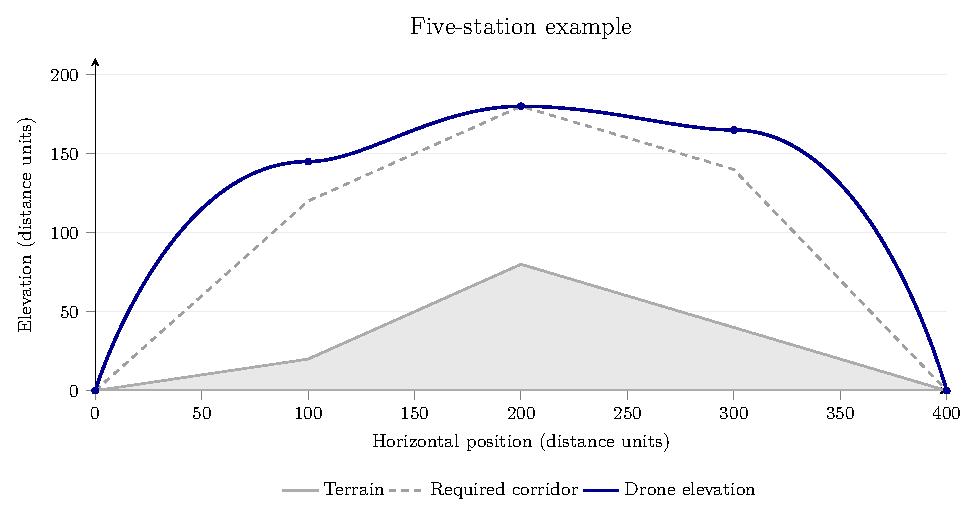
\includegraphics[width=.98\linewidth]{figures/example.pdf}
\caption{The five-station example.  Clearance is measured at horizontal position.  The first and last corridor segments contain takeoff and landing ramps.}
\label{fig:example}
\end{figure}

The drone branch\textquotesingle s \path{task.md} reports tests of 48 accepted WASM routes against an independent graph planner, four empty or rejected inputs, and 12 native Lean/WASM comparisons.  Earlier checks included exhaustive short-route optima, translated and reversed terrain, and sampled continuous bounds.  Those test drivers and raw logs belonged to the development workspace and were excluded from its committed scope.  These results are retained here as attributed development evidence.  The committed Lean theorems provide the inspectable universal statements.

The same record reports a fresh compiler/model comparison followed by the specification build on September 26, 2026.  It also states that the binary was outside the committed artifact packages and that the drone registration used by that local check was excluded from the commit.  Consequently, reproduction from the committed branch uses the explicit Lean targets below.  The report-specific build of \path{Project.Drone.Spec} and \path{Project.Drone.SourceChecks} passed on September 26, 2026.  A separate audit of the principal source, allocation, and execution theorems lists only \path{propext}, \path{Classical.choice}, and \path{Quot.sound}, as applicable.  A freshly compiled module also reproduced all five report examples in Wasmtime, with exact native Lean agreement.

\begin{lstlisting}
tools/leanrun --timeout 15m lake -q -d proofs/talos/lean build \
  Project.Drone.Spec Project.Drone.SourceChecks

tools/leanrun --timeout 2m lake env lean --run \
  test/DroneNative.lean 0 20 80 40 0
\end{lstlisting}

The pinned setup uses Lean 4.34.0-rc2 and the repository's Talos dependency.  The repository runner enforces the local resource policy and serializes Lean work.  The proof build checks the whole-flight source result and the compiled specification in the same dependency graph.  Its printed axiom dependencies allow review of the final result's logical assumptions.  Main's compiler theorem has its own \texttt{tools/arithmetic-check.js proof} command on that branch.  The compiler account uses main's theorem source and retained integration evidence.  The report-specific builds used the drone checkout.


\subsection{Fresh terrain runs}

Figures~\ref{fig:flat-plateau} and~\ref{fig:hill-ridges} show four additional runs of the compiled planner.  Each input contains 15 stations spanning 1,400 distance units.  The figures use the returned altitude and speed words, evaluated with the prescribed continuous primitives at 101 normalized times per segment.  Markers identify the returned waypoints.  The filled region is the piecewise-linear terrain, and the dashed curve is the required corridor.  The plotted horizontal coordinate follows the primitive's progress function.

Every returned word agrees with a separate native Lean invocation on the same input.  The report retains the complete inputs, both outputs, exact tick totals, and plotting samples in its figure data.  The four routes have the same time, $90{,}240/840=107\tfrac{3}{7}$ seconds, while their selected altitude excess differs.  In these cases the planner preserves the same waypoint-speed sequence and adjusts altitude to satisfy the terrain constraints.  Table~\ref{tab:runs} records the resulting secondary costs.  These new runs are distinct from the historical 15-station examples in the development record.

\begin{table}[htbp]
\centering
\begin{tabular}{lr}
\toprule
Terrain & Sampled altitude excess\\
\midrule
Flat & 0\\
Broad plateau & 300\\
Rounded hill & 850\\
Repeated ridges & 800\\
\bottomrule
\end{tabular}
\caption{Fresh compiled runs.  The secondary cost sums altitude offsets above the station floors.}
\label{tab:runs}
\end{table}

\begin{figure}[p]
\centering
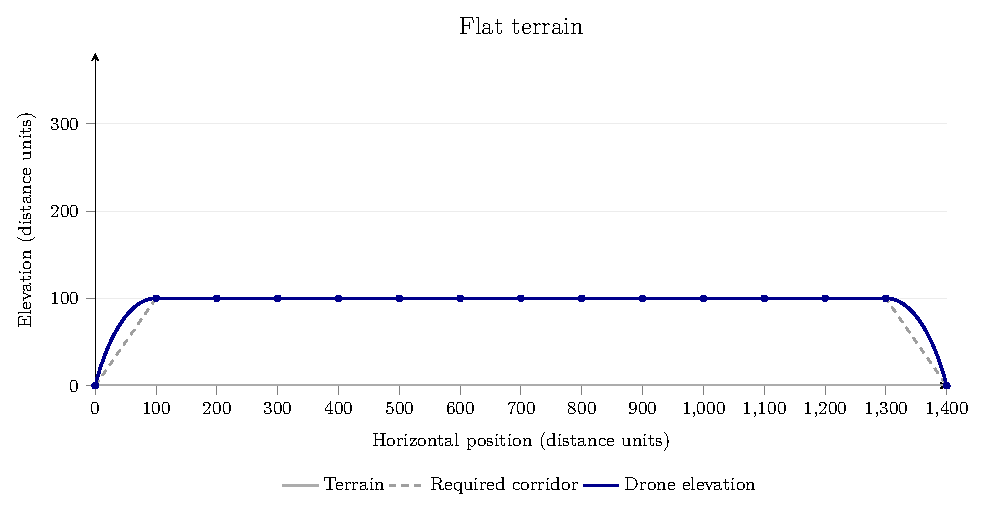
\includegraphics[width=.98\linewidth]{figures/flat.pdf}
\vspace{8mm}
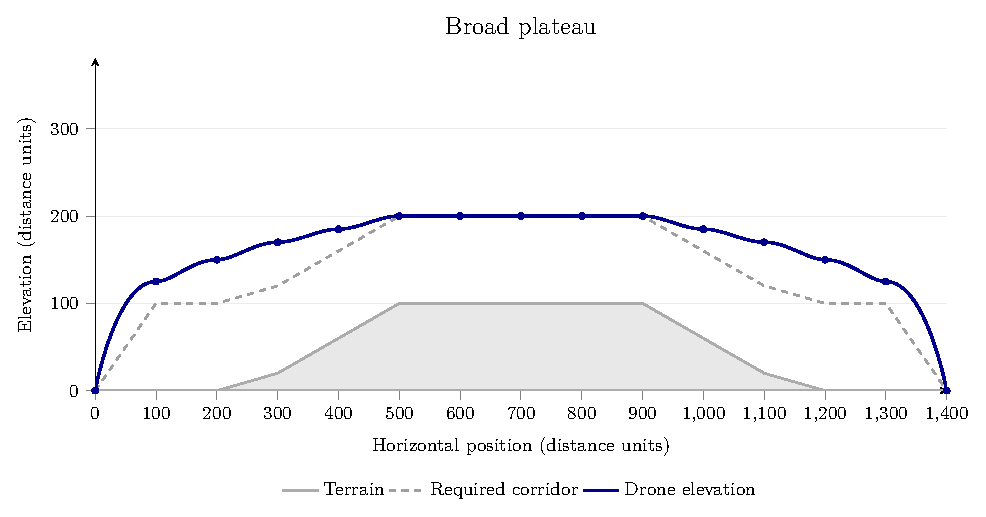
\includegraphics[width=.98\linewidth]{figures/plateau.pdf}
\caption{Fresh WASM outputs on flat terrain and a broad plateau.  The flat route follows the 100-unit interior floor.  The plateau route gains altitude before the rising terrain.  Native Lean returns the same waypoint words.}
\label{fig:flat-plateau}
\end{figure}

\begin{figure}[p]
\centering
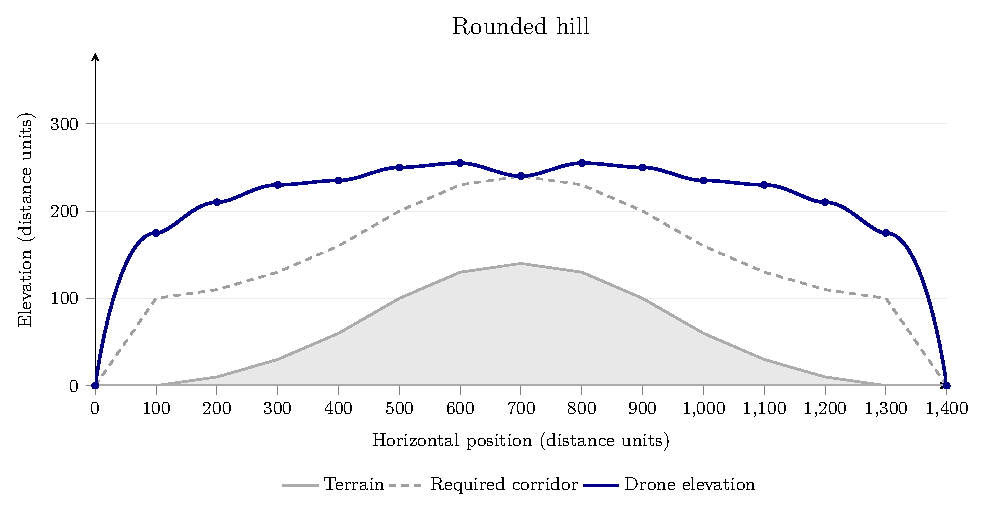
\includegraphics[width=.98\linewidth]{figures/hill.pdf}
\vspace{8mm}
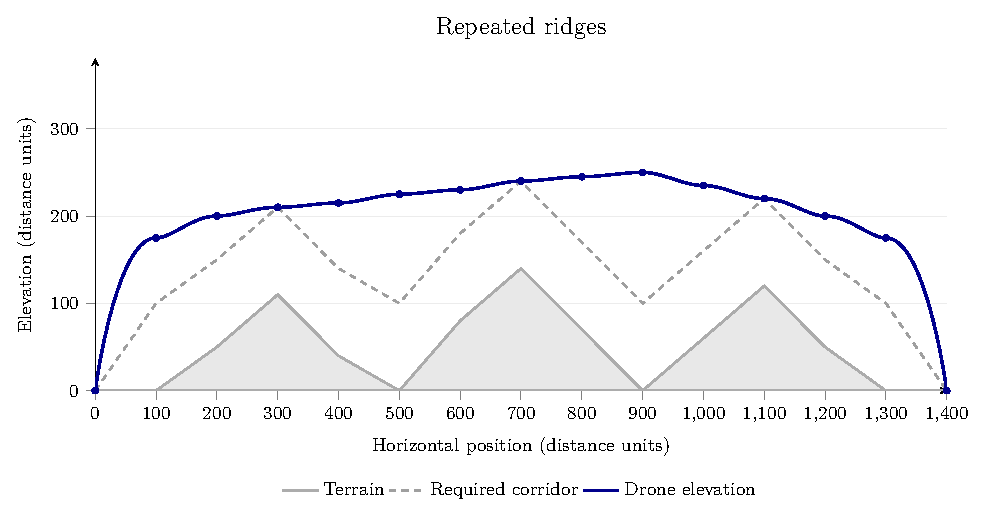
\includegraphics[width=.98\linewidth]{figures/ridges.pdf}
\caption{Fresh WASM outputs on a rounded hill and repeated ridges.  The planner selects a path above the corridor where doing so preserves traversal time.  All four 15-station plots share the same axis limits.}
\label{fig:hill-ridges}
\end{figure}

\clearpage

\section{Assumptions, remaining work, and related methods}
\label{sec:limits}

The result assumes an ideal point mass with exact piecewise-linear terrain and exact execution of the returned interpolation.  Terrain errors, state-estimation errors, delays, wind, tracking error, and coupled acceleration authority would change the safety problem.  The present clearance corridor also fixes specific takeoff and landing ramps.  A safety theorem for a physical vehicle would need to relate those additional quantities to the trajectory and its reserved margins.

The graph's finite state choices and primitive family determine optimality.  The secondary cost sums altitude excess at stations.  The conservative Bernstein certificate may remove safe continuous edges from consideration.  The all-stop witness establishes existence within this graph even for steep accepted terrain, at the cost of longer travel time.  Claims about a larger continuous control problem require a relation between that problem and the finite graph.

The generated-model proof establishes exact execution under explicit heap conditions.  A complete drone binary package would additionally prove decoding, validation, and equality between the decoded binary and \path{Project.Drone.module}.  The main-branch general compiler result gives those connections for its admitted arithmetic language.  Extending that theorem to the drone's heap arrays and recursive call structure is another possible route, with a broader proof obligation.  Host marshaling and the native WASM engine remain external execution assumptions in either approach.

Finite motion primitives and dynamic programming are established planning methods~\cite{lavalle}.  This development fixes a small primitive family so that exact word arithmetic, continuous polynomial safety, and compiled execution can be connected in one proof chain.  Its contribution is that connection for the implemented planner and its returned array.

\appendix
\section{Claim-to-theorem guide}

All drone names in Table~\ref{tab:theorems} are relative to \path{Project.Drone}.  The source is \path{LeanExe/Examples/Drone.lean}, and the proof statements and dependencies are in \path{proofs/talos/lean/Project/Drone/}.  Compiler results use the \path{Project.Compiler.ArithmeticModule} namespace in main\textquotesingle s \path{proofs/talos/lean/Project/Compiler/SourceCorrectness.lean}.  The report\textquotesingle s companion files retain source revisions, proof-audit output, run inputs and outputs, and figure data.

\small
\begin{longtable}{>{\raggedright\arraybackslash}p{.31\linewidth}>{\raggedright\arraybackslash}p{.63\linewidth}}
\caption{Theorem endpoints used by the report.}\label{tab:theorems}\\
\toprule
Claim & Declaration\\\midrule
\endfirsthead
\toprule Claim & Declaration\\\midrule\endhead
Ceiling square root & \path{Sqrt.ceilSqrt_correct}\\
Rest duration bounds & \path{Arithmetic.restSeconds_bounds}\\
Continuous accepted-edge clearance & \path{Edges.state_edge_clearance}\\
Exact moving duration in ticks & \path{Timing.state_ticks_exact}\\
Non-wrapping predecessor costs & \path{Costs.predecessor_exact}\\
Executable row optimum & \path{Planner.advance_correct}, \path{Planner.layers_optimal}\\
Accepted-input feasibility & \path{Feasibility.all_stop_flight}, \path{Feasibility.terrain_terminal_optimal}\\
Parent-history correspondence & \path{History.computed_history_valid}\\
Output feasibility and optimality & \path{Output.unwind_words}, \path{Output.compute_correct}\\
Rejected input and endpoints & \path{Output.compute_invalid}, \path{Output.compute_empty}, \path{Output.compute_endpoints}\\
Global position and velocity & \path{Trajectory.compute_global_smooth}\\
Spatial corridor identification & \path{Corridor.height_on_segment}, \path{Corridor.compute_spatial_segment}\\
Every-time flight coverage & \path{WholeFlight.compute_normalized_cover}\\
Whole-flight safety & \path{WholeFlight.compute_safe}\\
Global acceleration bounds & \path{WholeFlight.compute_acceleration_away_from_joins}, \path{Trajectory.compute_global_acceleration_within}\\
Allocation bound & \path{Execution.computeCost_bound}\\
Exact compiled output and heap & \path{Execution.compute_exact}\\
Public compiled result & \path{Spec.compute_correct}, \path{Spec.compute_safe}\\
General compiler admission and correctness & \path{compileEnvironment_correct}\\
Successful compilation implies correctness & \path{compileEnvironment_sound}\\
\bottomrule
\end{longtable}
\normalsize

\begingroup
\small
\bibliographystyle{plain}
\bibliography{references}
\endgroup
\end{document}
